\documentclass[conference]{IEEEtran}
\IEEEoverridecommandlockouts

\usepackage{cite}
\usepackage{amsmath,amssymb,amsfonts}
\usepackage{graphicx}
\usepackage{textcomp}
\usepackage{xcolor}
\usepackage{url}

\graphicspath{{figures/}}

\begin{document}

\title{Actuator-Constrained Early Intention Prediction for Simulated Rock-Paper-Scissors Robot Hands}

\author{\IEEEauthorblockN{Mingyu Cho}
\IEEEauthorblockA{\textit{Embodied Artificial Intelligence Final Project}\\
\textit{Hanyang University}\\
Seoul, Republic of Korea}}

\maketitle

\begin{abstract}
This report presents a screen-rendered robot-hand counterattack demo for Rock-Paper-Scissors. The task is framed as actuator-constrained early intention prediction: the system observes a prompt-window human hand motion, predicts the intended final gesture before the window closes, selects the winning counter move, and accepts the episode only when the simulated hand can reach the counter pose within the actuator deadline. The final live demo uses a frozen v4 skeleton predictor with profile weights $[0.25, 0.75, 0.0]$, while v7e is retained only as a diagnostic branch after failing strict original20 validation at $17/20$. In the selected final live take, the human performs rock during the final prompt window, the system issues robot paper, and the actuator feasibility checker reports an actuator-feasible win with $0.4667$ s remaining.
\end{abstract}

\begin{IEEEkeywords}
early action prediction, skeleton sequence modeling, actuator feasibility, robot hand, Rock-Paper-Scissors, SCHUNK SVH
\end{IEEEkeywords}

\section{Introduction}

Fast human-robot interaction is not only a perception problem. A robot can predict the correct future action and still fail if the decision arrives too late for the actuator to respond. This final project studies that timing gap through a compact Rock-Paper-Scissors task. The robot observes a human hand during a bounded prompt window and tries to issue a simulated counter gesture before the deadline.

The central question is: when does partial hand-motion evidence become useful early enough for an embodied response? This differs from final-frame gesture recognition. The system must decide from incomplete motion, abstain or wait when evidence is insufficient, and then verify that the selected counter gesture is reachable from the robot's start pose under velocity and deadline constraints.

The final implementation uses a skeleton-first pipeline. MediaPipe-style 21-landmark hand observations are converted into canonical landmark and velocity features, a frozen v4 temporal predictor estimates the final gesture, a counter policy maps the prediction to the winning robot gesture, and a kinematic SCHUNK-style hand renderer visualizes the response. Fig.~\ref{fig:pipeline} summarizes the final system.

\begin{figure}[t]
    \centering
    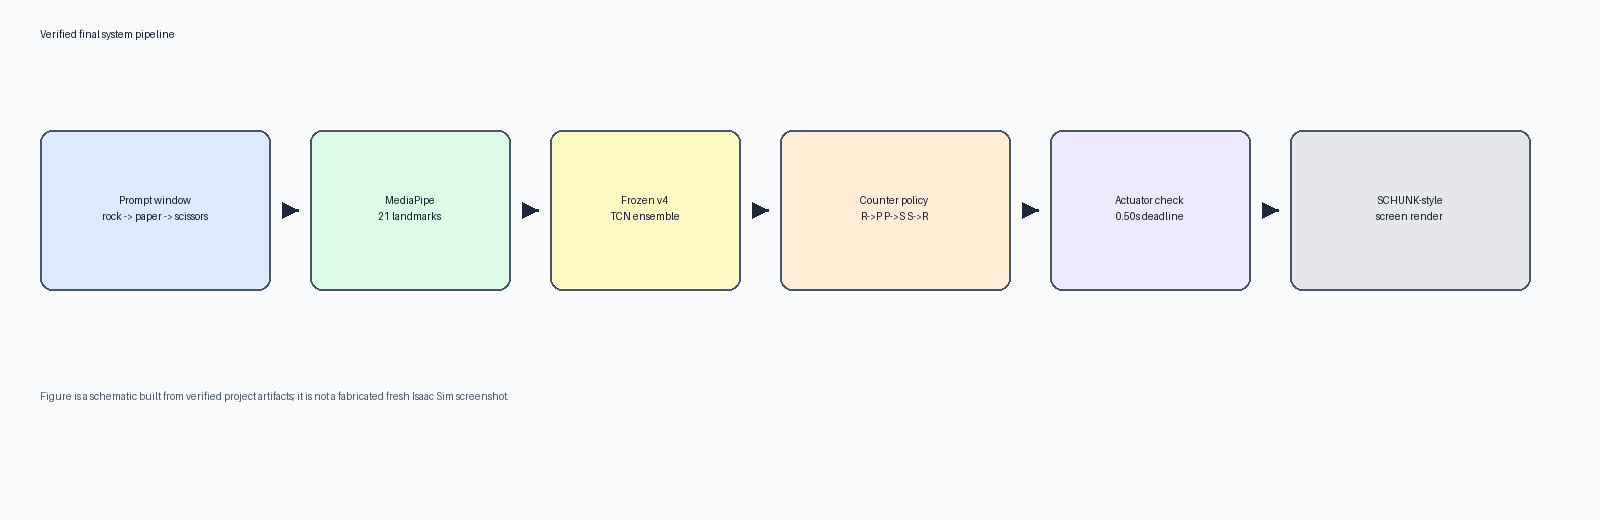
\includegraphics[width=\linewidth]{verified_system_pipeline.png}
    \caption{Final submission pipeline. This is a schematic built from verified project artifacts, not a fabricated fresh Isaac Sim screenshot.}
    \label{fig:pipeline}
\end{figure}

The contributions are:
\begin{itemize}
    \item a prompt-window RPS counterattack demo that preserves the temporal sequence \texttt{rock -> paper -> scissors} and acts only in the final response window;
    \item a frozen v4 fallback predictor policy for live/demo use, with v7e preserved as diagnostics instead of being promoted after strict-gate failure;
    \item an actuator-feasible episode criterion that combines prediction, counter selection, remaining time, velocity limits, and joint limits;
    \item a verified screen-rendered final live take and supporting three-take review artifact.
\end{itemize}

\section{Related Work}

Early action prediction studies recognition before the full action has been observed. Surveys and skeleton-action-prediction work emphasize that partial observation is a distinct problem from ordinary completed-action recognition \cite{kong2018survey,ke2019latent}. This project uses that framing but narrows the domain to prompt-conditioned hand motion, where the relevant information is not only the final hand shape but also the transition timing.

The learned predictor is intentionally lightweight. GRU and TCN-style temporal models are natural baselines for short sequential signals because they model temporal context without requiring raw video processing \cite{chung2014gru}. In this project, raw camera frames are used for capture and overlay, while the predictor consumes canonical skeleton features. This follows the project boundary of skeleton ground truth first.

The system also borrows from selective prediction and calibration. A model should not always act merely because it has a nonzero preferred class. Selective classification and confidence calibration work motivate the use of confidence thresholds, margins, confirmation counts, and response-window gates \cite{geifman2017selective,guo2017calibration}. The final metric then adds an embodied layer: a confident prediction must still be actuator feasible.

Isaac Sim and Isaac Lab provide the target simulation context for articulated robot assets and actuator modeling \cite{isaacsim,isaaclabactuators}. In this submission, archived SCHUNK/Isaac render evidence is used as verified visual material, and the final live demo uses a local SCHUNK-style kinematic renderer as the fallback screen-rendered hand.

\section{Method}

\subsection{Prompt-Window Observation}

Each live take follows a fixed prompt sequence:
\[
\texttt{rock} \rightarrow \texttt{paper} \rightarrow \texttt{scissors}.
\]
The response window is the final \texttt{scissors} prompt. For the selected final take, the human target gesture is rock, but it is still performed during the final \texttt{scissors} response window. This prevents the clip from becoming a generic gesture video and keeps the temporal structure consistent with the intended demo protocol.

\subsection{Skeleton Predictor}

The final live/demo predictor is frozen to v4. The operational config is the rock-guard v4 realtime selector config under \texttt{configs/}. It combines three profile slots:
\[
w = [0.25, 0.75, 0.0],
\]
corresponding to \texttt{v4\_fewshot\_aug\_tcn}, \texttt{v4\_rebalanced\_tcn}, and \texttt{v4\_final\_gate\_micro}. The third profile is retained in the config surface but has zero live/demo weight. The policy uses confidence threshold $0.70$, margin threshold $0.10$, confirmation count $2$, binary transition threshold $0.60$, and response prompt \texttt{scissors}.

Fig.~\ref{fig:tcn} shows the provided temporal convolution diagram used to explain the sequence model intuition.

\begin{figure}[t]
    \centering
    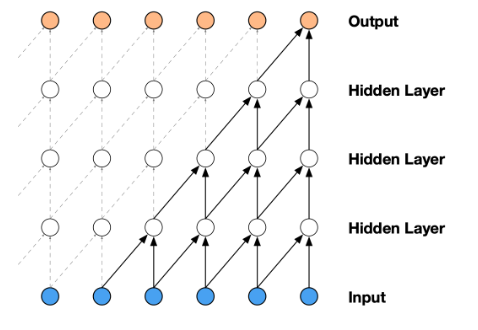
\includegraphics[width=0.85\linewidth]{tcn_temporal_model.png}
    \caption{Temporal convolutional model intuition for sequence-to-class prediction. The final implementation uses skeleton landmark and velocity features rather than raw images as predictor input.}
    \label{fig:tcn}
\end{figure}

\subsection{Counter Policy and Actuator Feasibility}

The counter policy is deterministic: rock maps to robot paper, paper maps to robot scissors, and scissors maps to robot rock.
The robot starts from rock. After a confirmed response-window prediction, the feasibility checker evaluates whether the target counter pose can be reached from rock before the deadline. The final configuration uses a response delay of $0.08$ s, a deadline of $0.50$ s, normalized curl-joint limits $[0,1]$, and the velocity limits from the local kinematic RPS config.

The episode is counted as a success only if the prediction is correct, the counter move wins, joint limits are satisfied, and the required motion completes before the remaining deadline.

\section{Implementation}

The implementation is packaged under \texttt{src/embodied\_rps}. The final live recording workflow is exposed through a recording CLI, and the final submission support assets are generated by a separate asset-builder CLI. Exact commands are listed in the repository README.
This builder writes the dataset inventory, submission manifest, notebook, and report figures. It also rejects two common failure modes: claiming a replay rehearsal video as the final demo and writing local Windows absolute paths into durable submission text.

Fig.~\ref{fig:schunk} shows verified archived SCHUNK-style render keyframes. These images are reused as visible robot-hand style assets in the final screen-rendered overlay.

\begin{figure}[t]
    \centering
    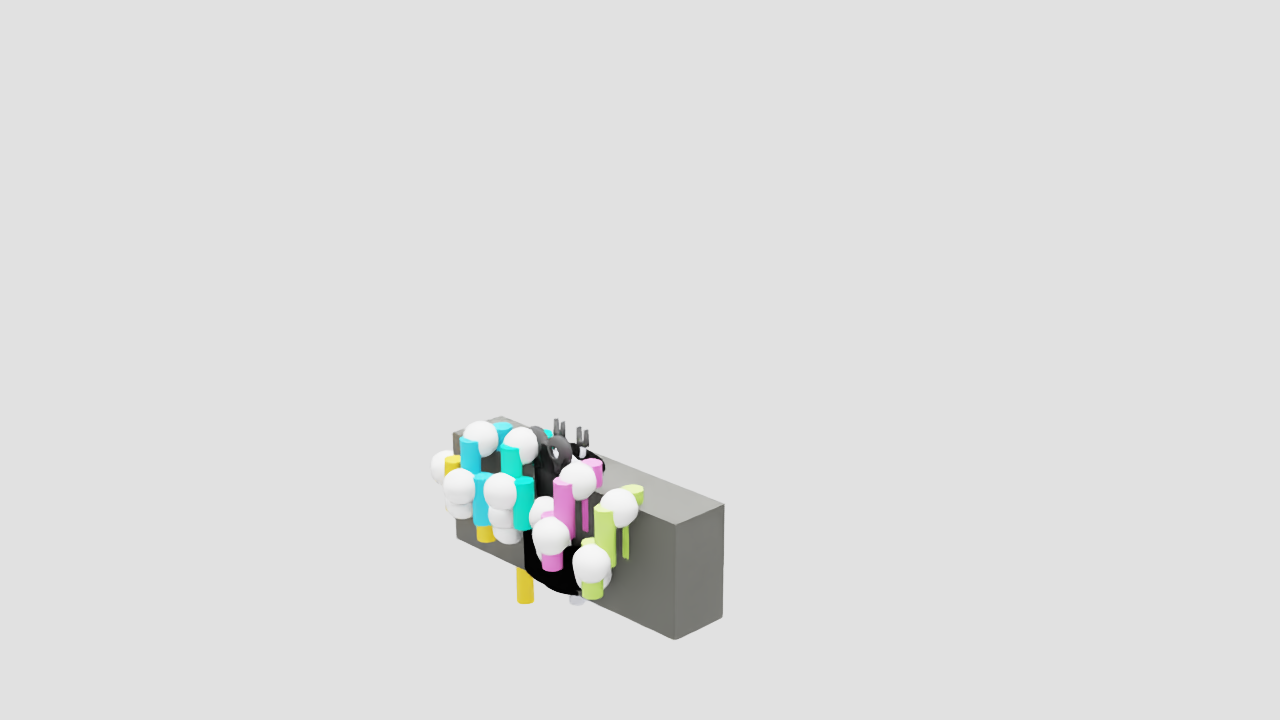
\includegraphics[width=0.31\linewidth]{schunk_rock_yaw45_pitch20.png}
    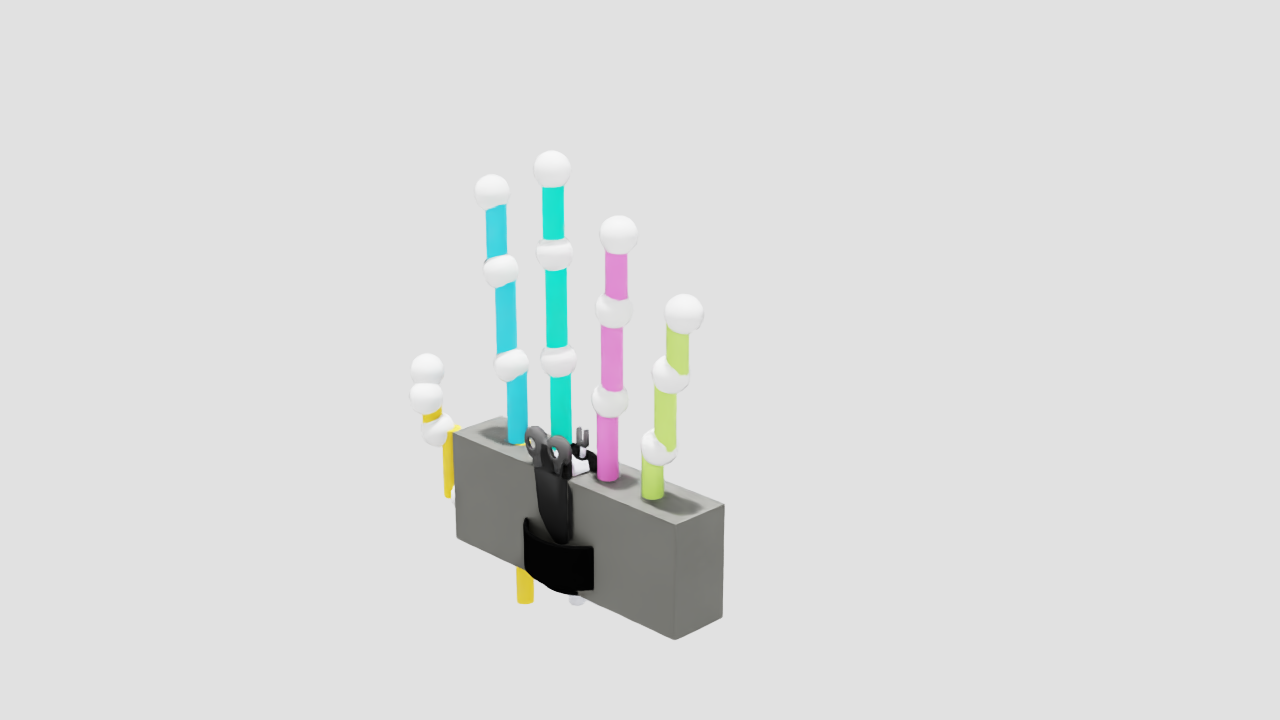
\includegraphics[width=0.31\linewidth]{schunk_paper_yaw45_pitch20.png}
    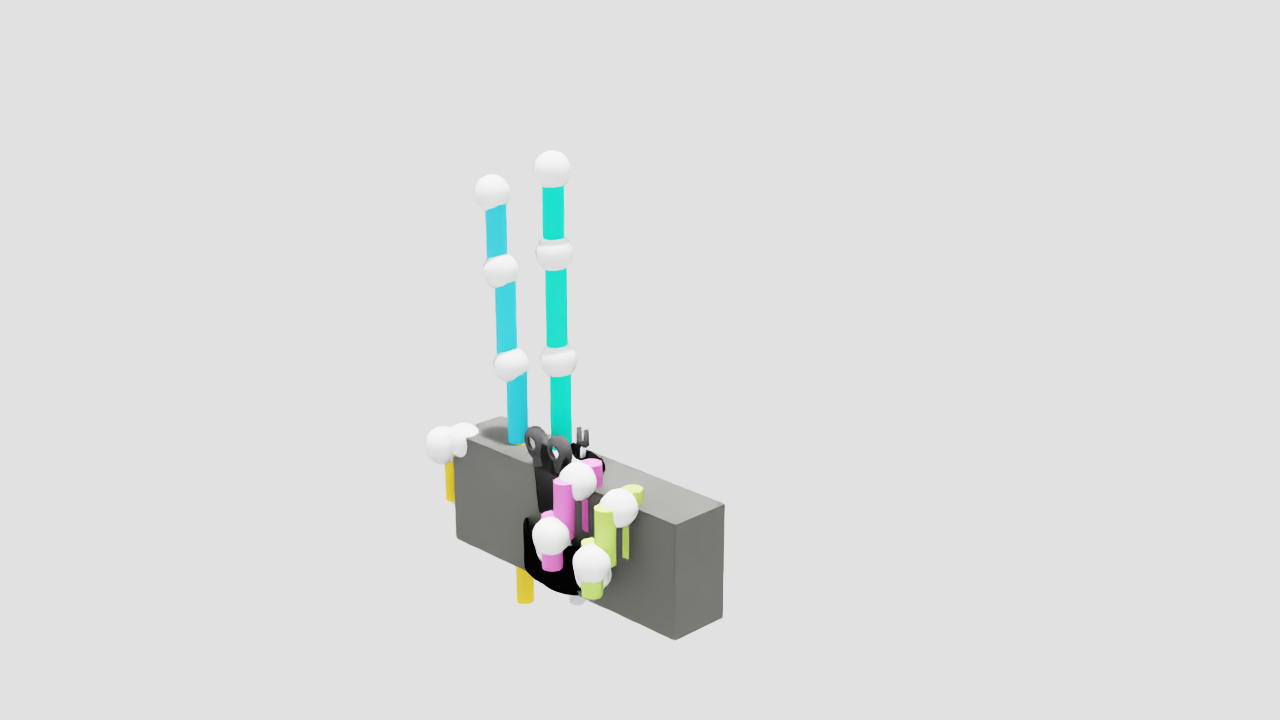
\includegraphics[width=0.31\linewidth]{schunk_scissors_yaw45_pitch20.png}
    \caption{Verified archived SCHUNK-style render keyframes for rock, paper, and scissors. These are archived evidence images, not newly fabricated report graphics.}
    \label{fig:schunk}
\end{figure}

\section{Results}

Table~\ref{tab:metrics} summarizes the final live/demo policy and diagnostic outcomes. The v4 fallback remains the only live/demo policy. The v7e branch is report evidence only: it improved some paper-transition behavior but failed strict original20 validation and was therefore not promoted.

\begin{table}[t]
\caption{Final Policy and Demo Metrics}
\label{tab:metrics}
\centering
\scriptsize
\begin{tabular}{p{0.27\linewidth}p{0.28\linewidth}p{0.32\linewidth}}
\hline
Category & Metric & Value \\
\hline
v4 fallback & profile weights & $[0.25,0.75,0.0]$ \\
v4 fallback & original20 strict & $20/20$ \\
v4 fallback & heldout15 validation & $11/15$ validation-only \\
v7e diagnostics & original20 strict & $17/20$, not promoted \\
Final live take & selected take & human rock -> robot paper \\
Final live take & episode result & actuator-feasible win \\
Final live take & remaining time & $0.4667$ s \\
\hline
\end{tabular}
\end{table}

The selected final live candidate is shown in Fig.~\ref{fig:finaltake}. It captures the final response window with the human target rock, the frozen v4 decision state, the robot counter paper, and the feasibility status. The visible hand panel uses archived SCHUNK-style render keyframes for the robot response.

\begin{figure}[t]
    \centering
    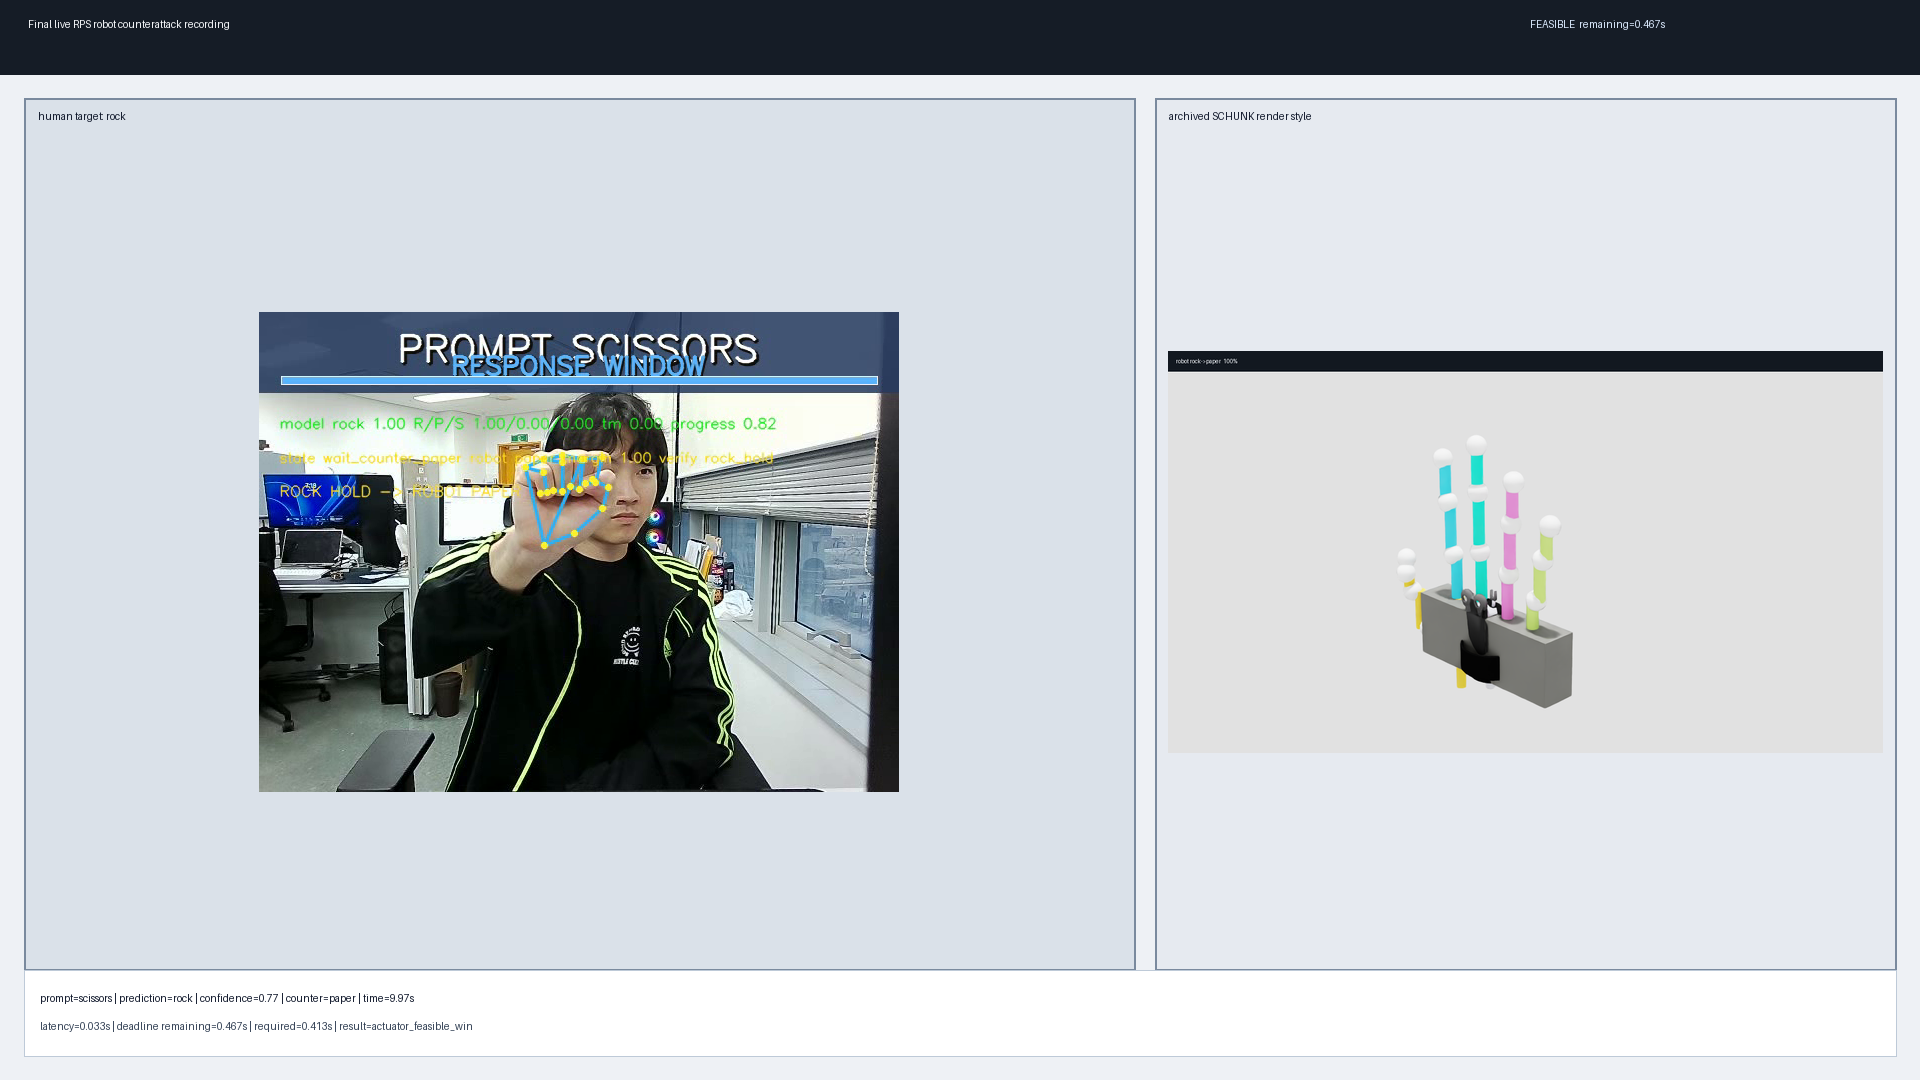
\includegraphics[width=\linewidth]{final_live_candidate_poster.png}
    \caption{Poster frame from the selected final live candidate. The frame shows the \texttt{PROMPT SCISSORS} response window, human target rock, robot counter paper, and feasible actuator result.}
    \label{fig:finaltake}
\end{figure}

The three-take review compilation is retained as supporting evidence. It contains the passed selected rock-to-paper take, a diagnostic paper-to-scissors take with no confirmed paper decision, and a diagnostic scissors-to-rock take that confirmed scissors but missed the actuator deadline.

\section{Discussion}

The final result supports the project framing: prediction quality alone is not enough. The selected live take succeeds because the response-window decision arrives early enough for the robot hand to move from rock to paper with time remaining. The failed diagnostic takes are equally important. A no-decision paper take demonstrates that the predictor can abstain or fail to stabilize, while the late scissors take demonstrates that a correct class decision can still fail under actuator timing.

The most important model decision was to preserve v4 as the live/demo fallback. Later v7 branches were useful research diagnostics, but strict validation failures prevented promotion. In particular, v7e reached $17/20$ on original20 after paper-transition rescue but introduced scissors-boundary failures. Promoting it would have weakened the final live demo even though it produced useful negative evidence for future work.

The main limitation is that the final demo is screen-rendered, not a closed-loop physical robot. The archived SCHUNK/Isaac evidence and local kinematic renderer are adequate for the course deliverable, but a future version should run the same prompt-window policy through a full Isaac articulation pipeline and then through real hardware or a higher-fidelity actuator model.

\section{Conclusion}

This project delivers a final live screen-rendered robot counterattack demo built around actuator-constrained early intention prediction. The system preserves the prompt-window temporal assumption, uses a frozen v4 skeleton predictor, maps predictions to counter gestures, checks actuator feasibility, and renders a SCHUNK-style robot response. The final candidate is an actuator-feasible win for human rock -> robot paper, while v7e remains a diagnostic branch rather than a promoted live model. Future work should target the residual paper/scissors boundary and move from the kinematic renderer toward full Isaac Sim articulation and hardware-grounded actuator validation.

\bibliographystyle{IEEEtran}
\bibliography{final_report}

\end{document}
